\documentclass[8pt]{beamer}
\usepackage{hyperref}
\usepackage[T2A]{fontenc}
\usepackage{pscyr}
\usepackage[english,russian]{babel}
\usepackage[utf8]{inputenc}
\usepackage{graphicx}
\setbeamertemplate{caption}[numbered]
\usetheme{CambridgeUS}
\beamertemplatesquareitem
\begin{document}
\title{Моделирование фильтра циклон}
\author{Дмитрий Богданов}
\institute{СПБГПУ}
\date{\today}
\frame{\titlepage}
\frame{\frametitle{Содержание}\small{\tableofcontents}}
\section{Постановка задачи}
\frame{\frametitle{Геометрия фильтра}
	\small{
		\hspace{0.02\textwidth}
		\begin{minipage}[t]{0.5\linewidth}
			\vspace{0.2\textwidth}
			\begin{table}[h]
			\caption{Геометрия фильтра}
			\hline
			\begin{tabular}{c c}
				\label{geometrytable}
				Диаметр цилиндра, $D$ & $0.205m$ \\
				Диаметр выходной трубы, $D_e$ & $0.5D$ \\
				Высота входного канала, $a$ & $0.5D$ \\
				Ширина входного канала, $b$ & $0.2D$ \\
				Длина выходной трубы, $h_e$ & $0.75D$ \\
				Полная высота фильтра, $H$ & $4.0D$ \\
				Высота цилиндра, $h$ & $1.5D$ \\
				Диаметр нижнего сечения фильтра, $B$ & $0.36D$ \\
			\end{tabular}
		\end{table}
	\end{minipage}
	\hfill
	\begin{minipage}[t]{0.45\linewidth}
		\centering
		\vspace{-1.5ex}
		\begin{figure}
			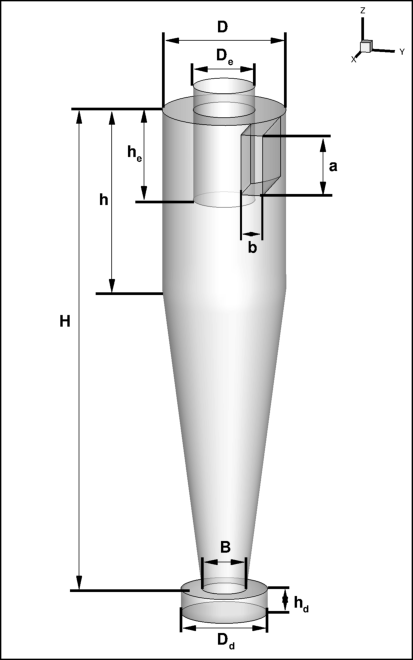
\includegraphics[scale=0.3]{Geometry}
			\caption{Схема фильтра}\label{fig:geometry}
		\end{figure}
	\end{minipage}
	}
}

\section{Определяющие уравнения}
\frame{
	\frametitle{Уравнения движения}
	\tiny{
		\begin{eqnarray}
			\nonumber
			\text{Уравнение неразрывности:} \\
			\frac{\partial \rho}{\partial t} + \nabla{(\rho \vec{V})}&=& 0, \\
			\hline
			\nonumber
			\\
			\nonumber
			\text{Уравнение баланса импульса:} \\
			\frac{\partial \rho \vec{V}}{\partial t} + \nabla{(\rho \vec{V} \vec{V})} &=& - \nabla{p} + \nabla{\left[(\mu + \mu_t) \nabla{\vec{V}}\right]} + \rho \vec{S_{V}}, \\
			\hline 
			\nonumber
			\\
			\nonumber
			\text{Уравнение баланса энергии:}\\
			\frac{\partial \rho h}{\partial t} + \nabla {(\rho \vec{V} h)} &=&  \frac{\partial p}{\partial t} + \nabla{\left[(\alpha + \alpha_t)\nabla{h}\right]} + \rho S_h, \quad \text{где } \alpha_t = \mu_t/Pr_t, \\
			\hline
			\nonumber
			\\
			\nonumber
			\text{Уравнение состояния:}\\
			p &=& \rho R T
		\end{eqnarray}
	}
}

\frame{
	\frametitle{Модель турбулентности}
		\tiny{
			\begin{eqnarray}
			\nonumber
			\text{Уравнение переноса кинетической энергии:} \\
			\nonumber
			\\
			\frac{\partial \rho k}{\partial t} + \nabla{(\rho \vec{V} k)} = P_k f_{rot} + \beta^* \rho k \omega + \nabla{\left[(\mu + \mu_t) \nabla k\right]}, \\
			\hline
			\nonumber 
			\\
			\nonumber
			\text{Уравнение переноса удельной скорости диссипации:} \\
			\nonumber
			\\
			\frac{\partial \rho \omega}{\partial t} + \nabla{(\rho \vec{V} \omega)} = \alpha \frac{\rho P_k }{\mu_t}f_{rot} -D_{\omega} + Cd_{\omega} + \nabla{\left[(\mu + \mu_t) \nabla \omega\right]}, \\
			\hline 
			\nonumber
			\\
			\nonumber
			\text{Поправка на кривизну линий тока:}\\
			\nonumber
			\\
			\nonumber
			f_{r1}(r^*,\tilde{r}) = 2r^*\left( \frac{1+C_{r1}}{1+ r^*} \right)\left[ 1-C_{r3}\arctan{(C_{r2}\tilde{r})} \right] - C_{r1}, \\
			\tilde{r} = 2\Omega_{ik}S_{kj}\frac{DS_{ij}}{Dt}\frac{1}{\Omega D^3}, \quad D^2 = \max(S^2, 0.09 \omega^2), \\
			\nonumber
			S^2 = 2 S_{ij}S_{ij}, \quad \Omega^2 = 2 \Omega_{ij} \Omega_{ij}, \quad r^* = S/\Omega, \\
			\nonumber
			C_{r1} = 1, \quad C_{r2} = 2, \quad C_{r3} = 1, \quad f_{rot} = \max[\min(f_{r1},1.25),0]
		\end{eqnarray}
  	}
}
\frame{
	\frametitle{Субстанциональная производная тензора скоростей деформации}
	\tiny{
		$$
			\tilde{r} = 2\Omega_{ik}S_{kj}\frac{DS_{ij}}{Dt}\frac{1}{\Omega D^3}
		$$
		Здесь субстанциональная производная тензора скоростей деформации равна
		\begin{equation}
			\mathbf{P} = \frac{DS_{ij}}{Dt} = div(\vec{V} \cdot \mathbf{S}),
		\end{equation}
		А суммирование компонент трёх тензоров по повторяющимся индексам явно расписывается как
		\begin{eqnarray}
			\nonumber
			\Omega_{ik}S_{kj}\frac{DS_{ij}}{Dt}=
			&\Omega_{xx} S_{xx} P_{xx} + \Omega_{xx} S_{xy} P_{xy} + \Omega_{xx} S_{xz} P_{xz} + \\
			\nonumber
			&\Omega_{yx} S_{xx} P_{yx} + \Omega_{yx} S_{xy} P_{yy} + \Omega_{yx} S_{xz} P_{yz} + \\
			\nonumber
			&\Omega_{zx} S_{xx} P_{zx} + \Omega_{zx} S_{xy} P_{zy} + \Omega_{zx} S_{xz} P_{zz} + \\
			\nonumber
			&\Omega_{xy} S_{yx} P_{xx} + \Omega_{xy} S_{yy} P_{xy} + \Omega_{xy} S_{yz} P_{xz} + \\
			&\Omega_{yy} S_{yx} P_{yx} + \Omega_{yy} S_{yy} P_{yy} + \Omega_{yy} S_{yz} P_{yz} + \\
			\nonumber
			&\Omega_{zy} S_{yx} P_{zx} + \Omega_{zy} S_{yy} P_{zy} + \Omega_{zy} S_{yz} P_{zz} + \\
			\nonumber
			&\Omega_{xz} S_{zx} P_{xx} + \Omega_{xz} S_{zy} P_{xy} + \Omega_{xz} S_{zz} P_{xz} + \\
			\nonumber
			&\Omega_{yz} S_{zx} P_{yx} + \Omega_{yz} S_{zy} P_{yy} + \Omega_{yz} S_{zz} P_{yz} + \\
			\nonumber
			&\Omega_{zz} S_{zx} P_{zx} + \Omega_{zz} S_{zy} P_{zy} + \Omega_{zz} S_{zz} P_{zz}
		\end{eqnarray}
	}
}
\frame{
	\frametitle{Модель частиц}
	\begin{minipage}[t]{0.6\linewidth}
		Уравнение движения частицы:
		\tiny{
			\begin{equation}
				\label{particle}
					m_p \frac{d \vec{V}_p}{dt} = \frac{1}{2}\rho |\vec{V}-\vec{V}_p|(\vec{V}-\vec{V}_p)\frac{d_p^2 \pi}{4}C_D + m_p \vec{g}\frac{\rho_l-\rho}{\rho_l} + \vec{F}_{\nabla{p}}
			\end{equation}
		}
		\tiny{
			\begin{table}[t]
				\begin{tabular}{r l}
					$m_p$ & -- масса частицы\\
					$\vec{V}_p$ & -- скорость частицы\\
					$\vec{V}$ & -- скорость жидкости\\
					$C_D$ & -- коэффициент сопротивления\\
					$\rho_l$ & -- плотность частицы (жидкой)\\
					$\rho$ & -- плотность жидкости \\
					$\vec{F}_{\nabla{p}}$ & -- сила, обусловленная действием на частицу градиента давлания
				\end{tabular}
			\end{table}
		}
		\begin{itemize}
			\item Cell-to-face-to-cell tracking для траекторий частиц.
			\item Если необходимы более детальные траектории используются дополнительные циклы решения внутри ячеек.
			\item Для решения уравнения (\ref{particle}) используется встроенный в OpenFOAM ODE солвер.
		\end{itemize}
	\end{minipage}
	\begin{minipage}[t]{0.3\linewidth}
		\vspace{0.3\textwidth}
		\begin{figure}
			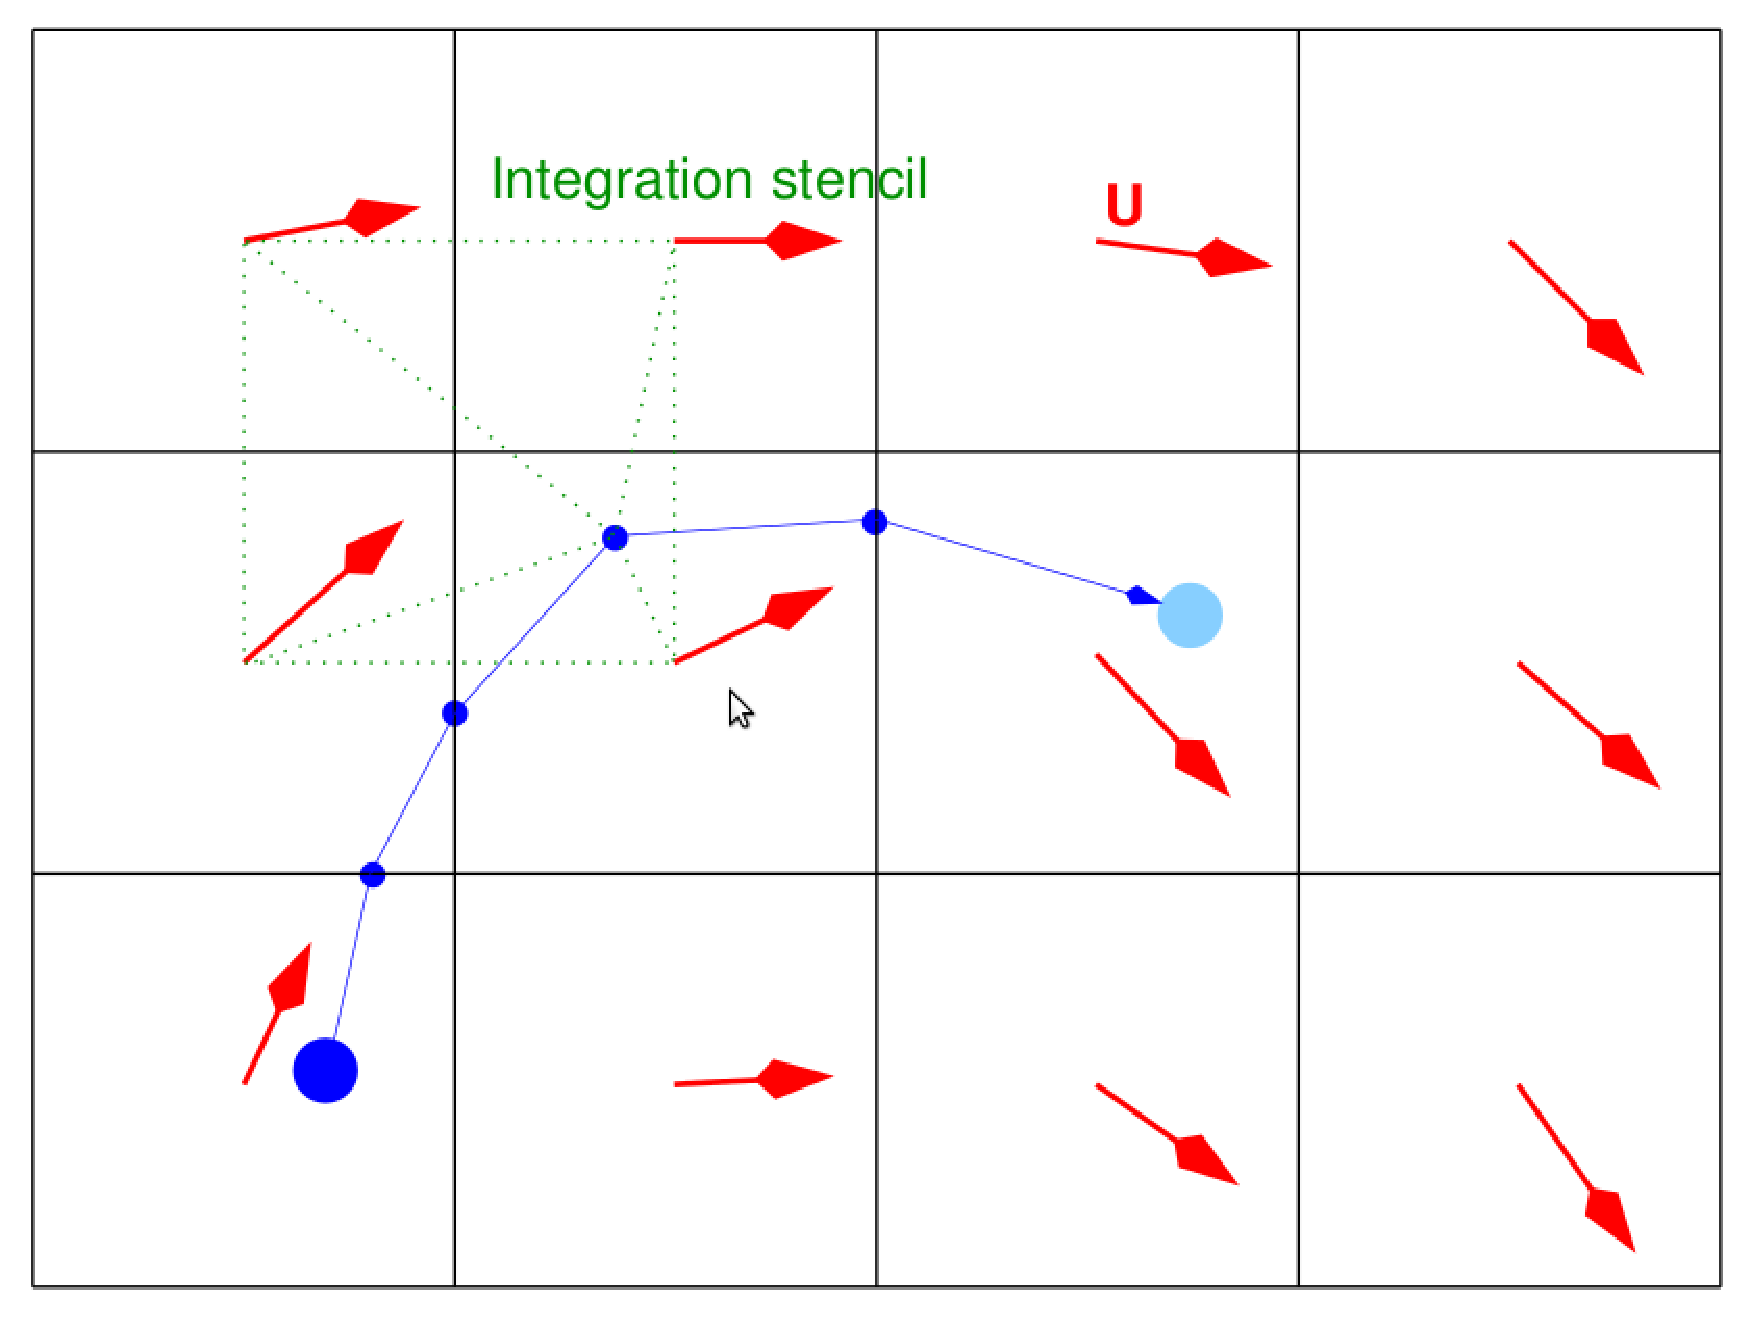
\includegraphics[scale=0.1]{particleJasak}
			\caption{Схема движения частиц}
		\end{figure}
	\end{minipage}
}

\section{Верификация модели турбулентности}
\frame{
	\frametitle{Течение в тестовом циклоне}
	\tiny{
	\begin{minipage}[t]{0.5\linewidth}
		\vspace{0.1\textwidth}
		\begin{table}[h]
			\caption{Параметры задачи о течении в тестовом циклоне}
			\hline
			\begin{tabular}{r c}
				Высота входного канала, $h_{in}$ & $0.2 [m]$ \\
				Высота выходного канала, $h_{out}$ & $0.2 [m]$ \\
				Ширина входного канала, $w_{in}$ & $0.1 [m]$ \\
				Ширина выходного канала, $w_{out}$ & $0.1 [m]$\\
				Высота циклона, $H_{full}$ & $0.4m$ \\
				Количество ячеек сетки, $nCells$ & $91440$ \\
				Массовый расход через входное сечение, $Q_{in}$ & $0.25 [kg/s] (V \approx 20 [m/s])$ \\
				Кинетическая энергия турбулентности на входе, $k_{in}$ & $10^{-5} [m^2/s^2]$ \\
				Удельная скорость диссипации на входе, $\omega_{in}$ & $1 [s^{-1}]$ \\
				Давление в выходном сечении, $p_{out}$ & $101325 [Pa]$ \\
				Температура во входном сечении, $T_{in}$ & $300 [K]$ \\
				Температура стенок, $T_{w}$, & $300 [K]$
			\end{tabular}
		\end{table}
	\end{minipage}
	\hspace{0.05\textwidth}
	\begin{minipage}[t]{0.35\linewidth}
		\centering
		\vspace{-1.5ex}
		\begin{figure}
			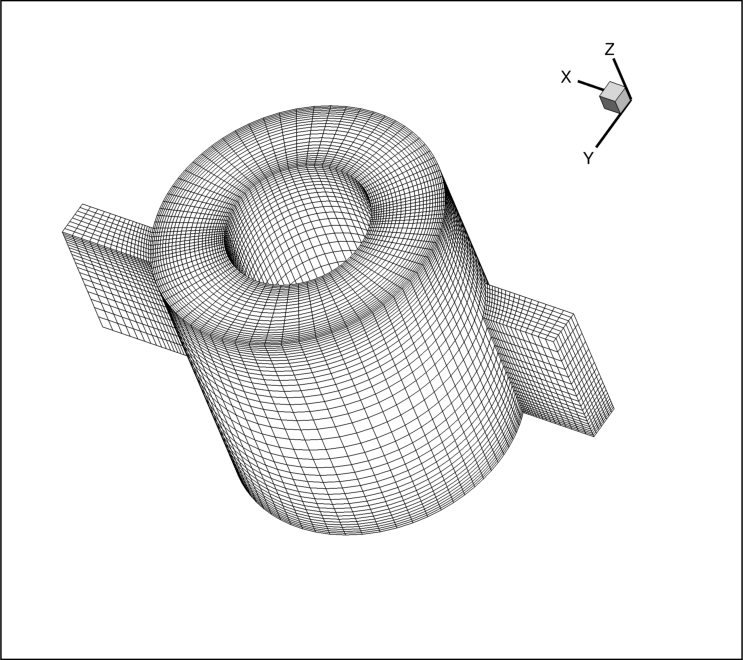
\includegraphics[scale=0.2]{swirlMesh}
			\caption{Сетка для задачи о течении в тестовом циклоне}\label{fig:verify}
		\end{figure}
	\end{minipage}
	}
}
\frame{
	\frametitle{Результаты верификации}
	\vspace{0.1\textwidth}
	\begin{minipage}[t]{0.45\linewidth}
		\begin{figure}
			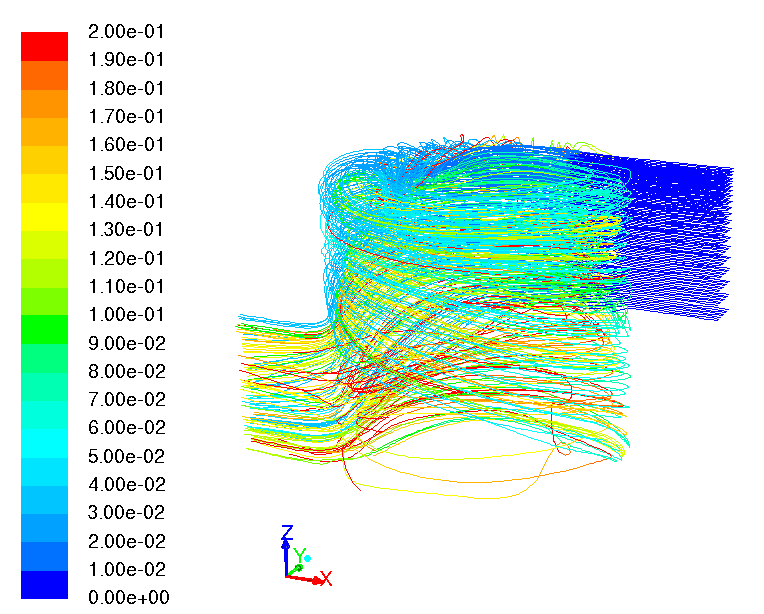
\includegraphics[scale=0.2]{testPathlines}
			\caption{Линии тока}
		\end{figure}
	\end{minipage}
	\hspace{0.05\textwidth}
	\begin{minipage}[t]{0.45\linewidth}
		\begin{figure}
			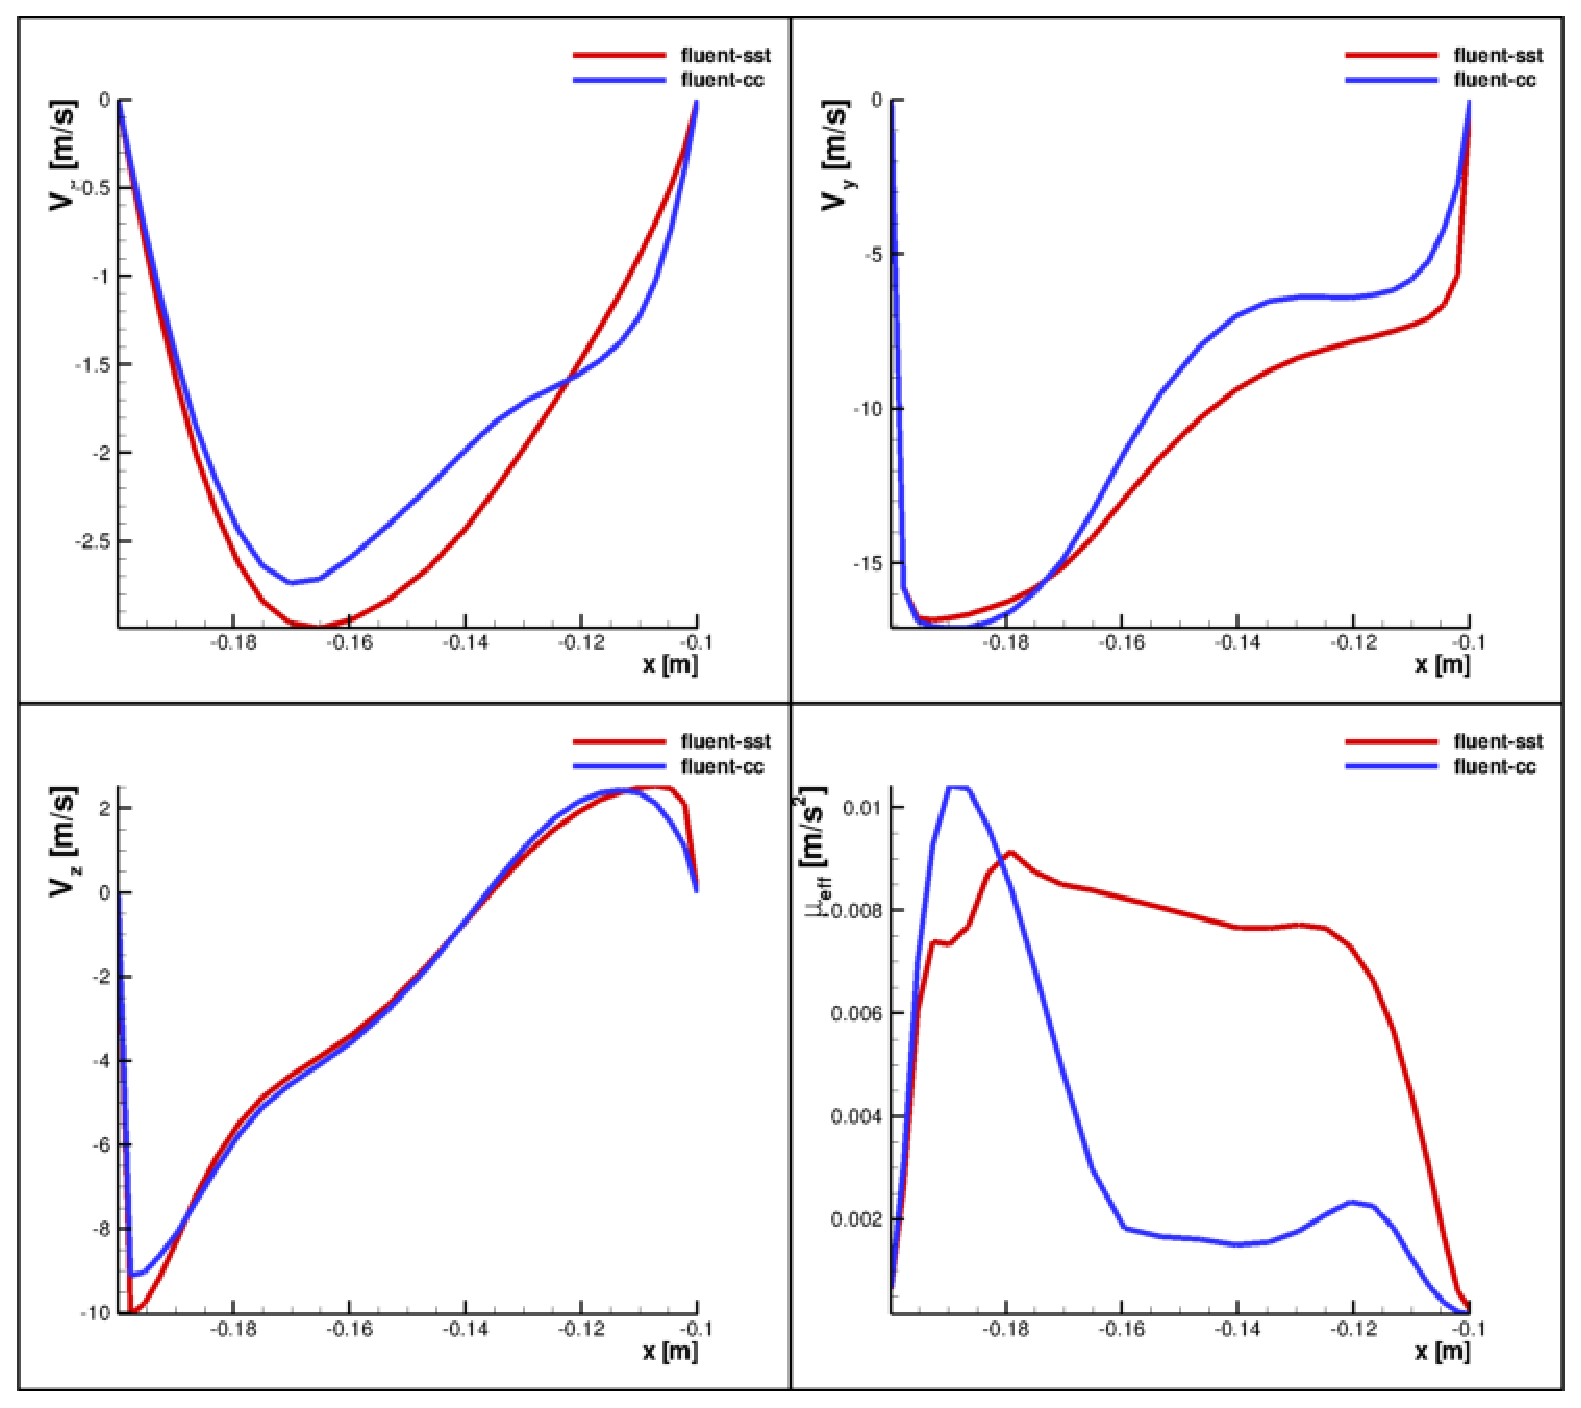
\includegraphics[scale=0.2]{Comparison}
			\caption{Влияние кривизны линий тока на профиль скорости}
		\end{figure}
	\end{minipage}
}

\section{Решение}
\frame{
	\frametitle{Граничные условия}\tiny{
	\begin{minipage}[t]{0.4\linewidth}
		\vspace{0.2\textwidth}
		\begin{table}
			\caption{Граничные условия}
			\hline
			\begin{tabular}{l c}
				Массовый расход через входное сечение, $Q_{in}$ & $0.08 [kg/s]$\\
				Температура газа на входе в циклон, $T_{in}$ & $300 [K]$ \\
				Температура внешних стенок, $T_w$ & $300 [K]$ \\
				Давление в выходном сечении, $p_{out}$ & $101325 [Pa]$ \\
				Внутренние стенки - адиабатические &
			\end{tabular}
		\end{table}
	\end{minipage}
	\hspace{0.05\textwidth}
	\begin{minipage}[t]{0.4\linewidth}
		\begin{figure}
			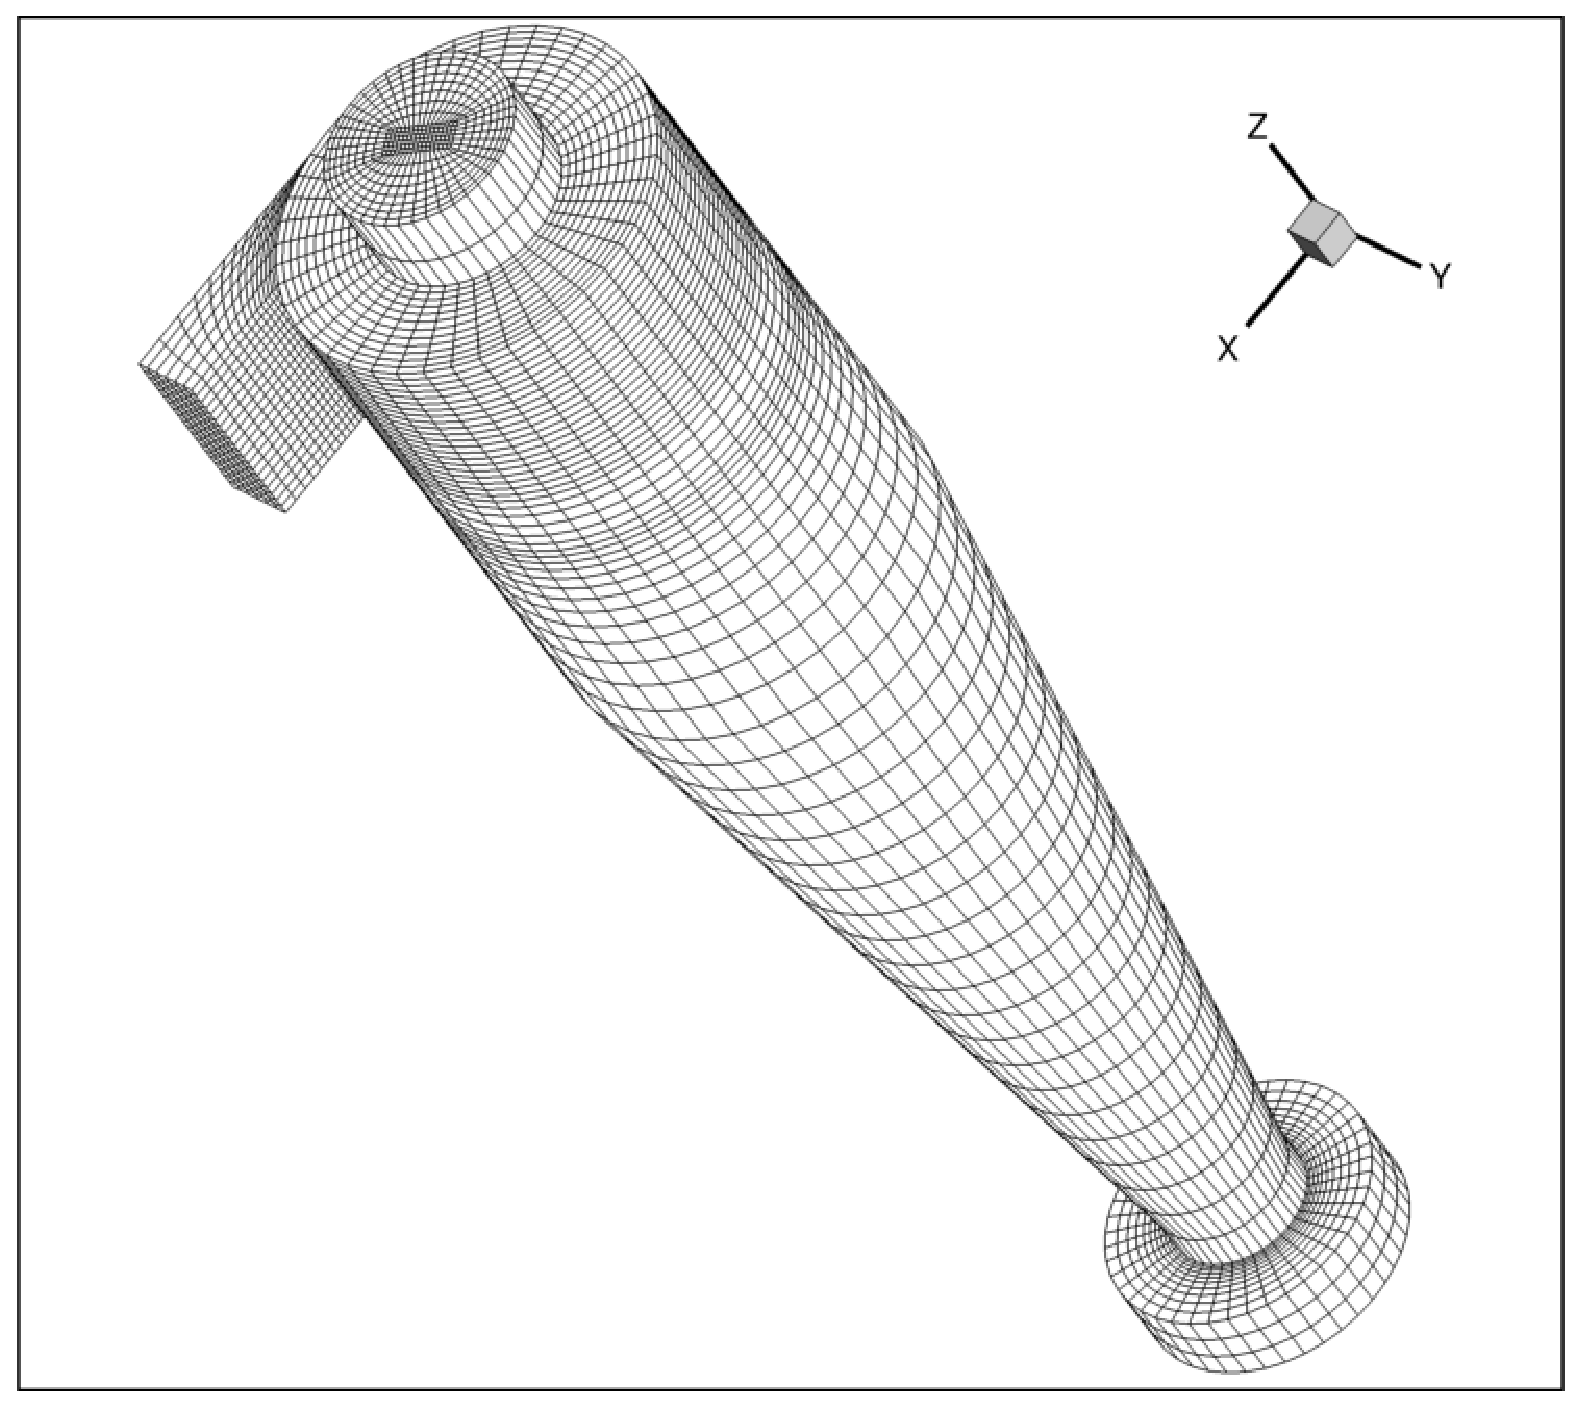
\includegraphics[scale=0.206]{Mesh}
			\caption{Сетка для реального фильтра}
		\end{figure}
	\end{minipage}
	}
}
\frame{
	\frametitle{SST без коррекции на кривизну}
	Расчёт для геометрии циклона, приведённой в таблице \ref{geometrytable} :
	\begin{minipage}[t]{0.4\linewidth}
		\begin{figure}
			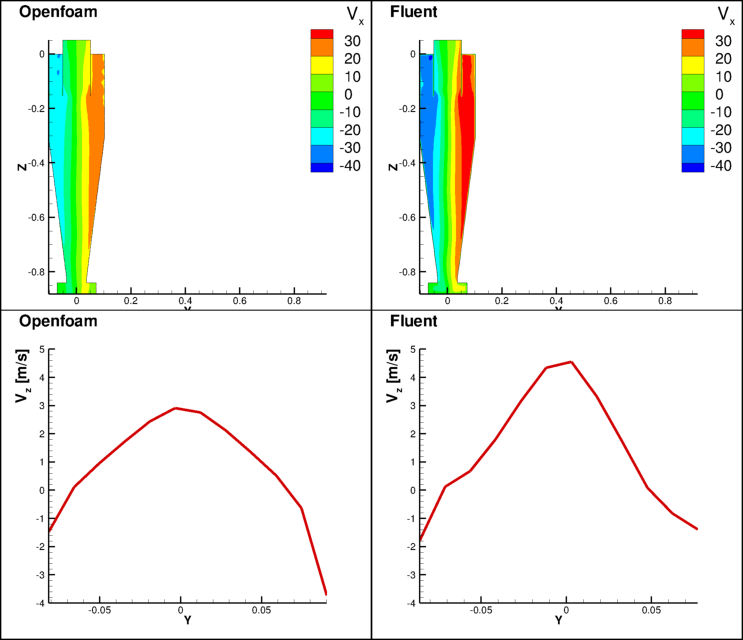
\includegraphics[scale=0.206]{Solution}
			\caption{Сравнение решения в OpenFOAM и FLUENT}
		\end{figure}
	\end{minipage}
	\hspace{0.05\textwidth}
	\begin{minipage}[t]{0.4\linewidth}
		\begin{figure}
			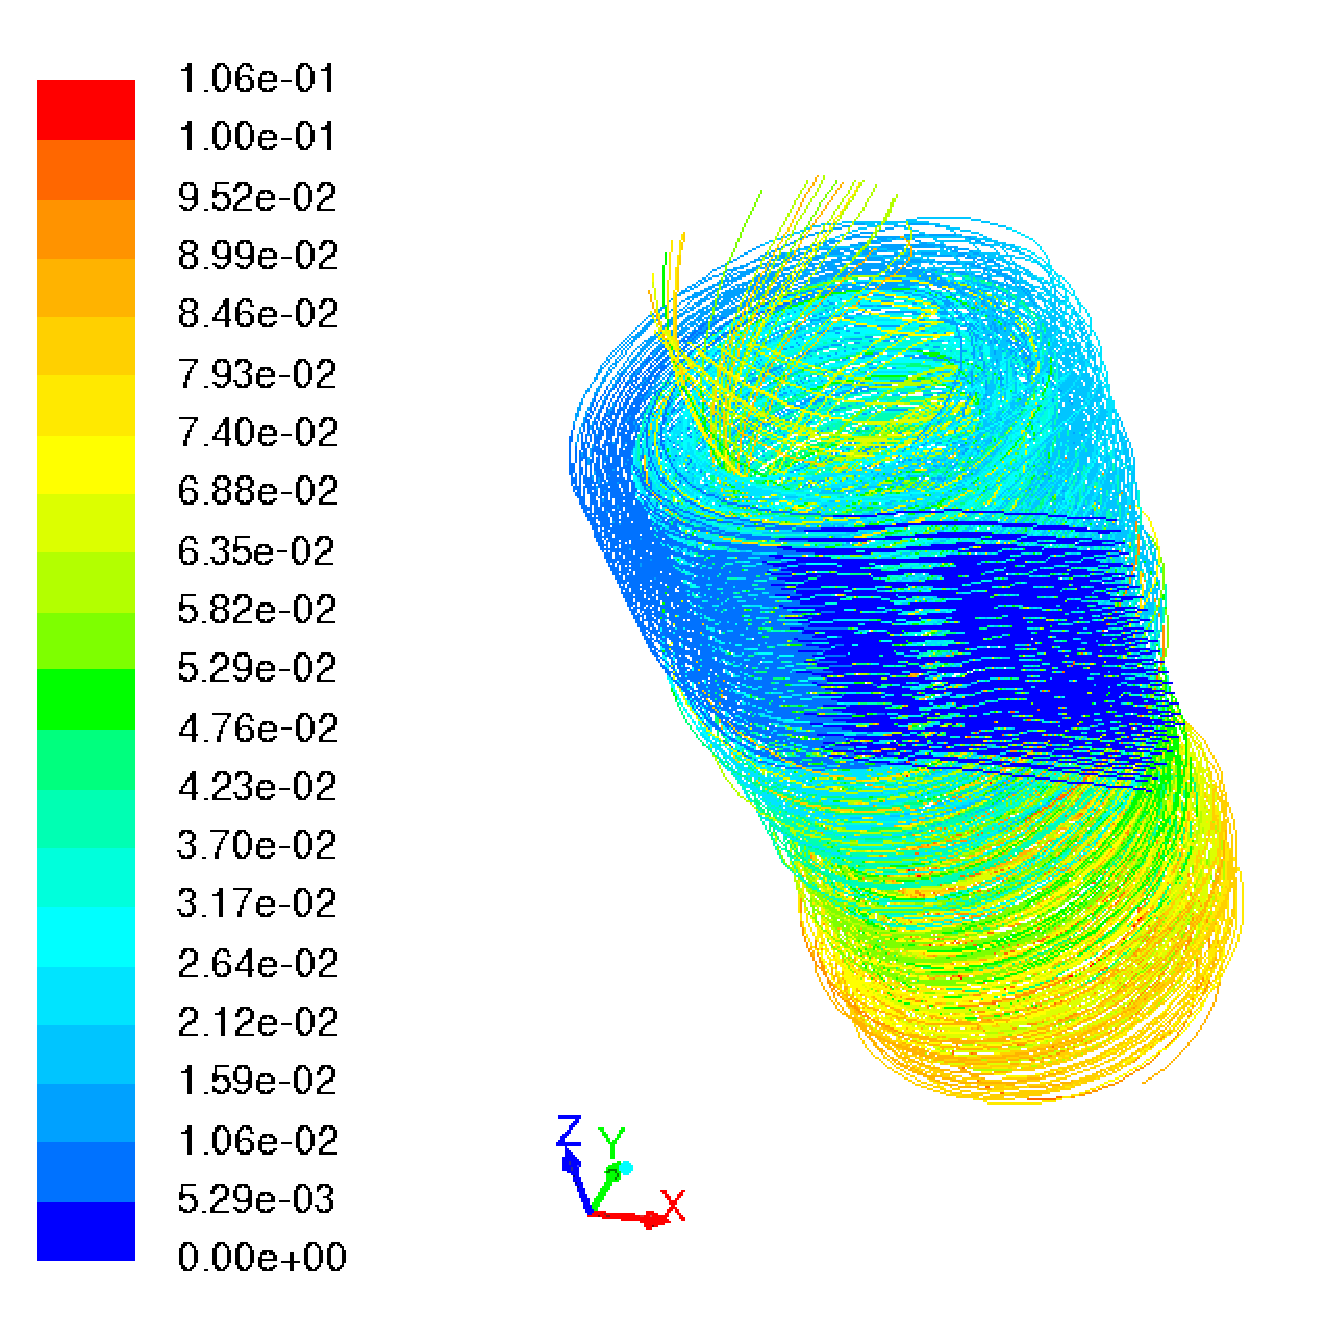
\includegraphics[scale=0.2]{Pathlines}
			\caption{Линии тока}
		\end{figure}
	\end{minipage}
}
\end{document}
